\documentclass[11pt,a4paper]{article}

\usepackage[margin=25mm]{geometry}
\usepackage[T1]{fontenc}
\usepackage[utf8]{inputenc}
\usepackage{lmodern}
\usepackage{amsmath}
\usepackage{amssymb}
\usepackage{booktabs}
\usepackage{tabularx}
\usepackage{array}
\usepackage{xcolor}
\usepackage{hyperref}
\usepackage{listings}
\usepackage{tikz}
\usetikzlibrary{arrows.meta,positioning,shapes.geometric,calc}
\setlength{\emergencystretch}{3em}

\hypersetup
{
    colorlinks=true,
    linkcolor=blue!55!black,
    urlcolor=blue!55!black,
    citecolor=blue!55!black
}

\definecolor{foamBlue}{RGB}{40,82,135}
\definecolor{foamGreen}{RGB}{54,125,82}
\definecolor{foamOrange}{RGB}{196,112,42}
\definecolor{foamRed}{RGB}{178,65,65}
\definecolor{codeBack}{RGB}{247,247,247}

\lstdefinestyle{foam}
{
    basicstyle=\ttfamily\small,
    backgroundcolor=\color{codeBack},
    frame=single,
    rulecolor=\color{black!20},
    breaklines=true,
    columns=fullflexible,
    keepspaces=true,
    showstringspaces=false,
    tabsize=4
}
\lstset{style=foam}

\newcommand{\code}[1]{\texttt{#1}}
\newcommand{\ddt}[1]{\frac{\partial #1}{\partial t}}
\newcommand{\grad}{\nabla}
\newcommand{\divergence}{\nabla \cdot}
\newcommand{\kappatensor}{\boldsymbol{\kappa}}
\newcommand{\heatflux}{\boldsymbol{q}}
\newcolumntype{Y}{>{\raggedright\arraybackslash}X}

\title{\textbf{anisotropicLaplacianFoam}\\
Beginner's Guide to Theory, Implementation, Execution, and Tutorial}
\author{OpenFOAM v2512 solver documentation}
\date{\today}

\begin{document}

\maketitle

\begin{abstract}
\code{anisotropicLaplacianFoam} is an OpenFOAM v2512 solver for transient heat
conduction in stationary solid materials with anisotropic thermal conductivity.
It solves temperature only. It does not solve fluid velocity, pressure,
advection, radiation, or conjugate heat transfer. This document explains the
physical model, the OpenFOAM implementation, the required input fields, the
execution workflow, and the included tutorial case
\code{tutorials/compositePlate2D}.
\end{abstract}

\tableofcontents
\newpage

\section{What the Solver Does}

The solver computes how temperature changes in a solid body when heat can
conduct through the material and when an optional internal heat source is
present. The most important feature is anisotropic conductivity: heat can move
more easily in one direction than another.

A common isotropic material uses one conductivity value, for example
$k=1.0~\mathrm{W/(m\,K)}$. An anisotropic material uses a tensor:

\[
\kappatensor =
\begin{bmatrix}
\kappa_{xx} & \kappa_{xy} & \kappa_{xz} \\
\kappa_{xy} & \kappa_{yy} & \kappa_{yz} \\
\kappa_{xz} & \kappa_{yz} & \kappa_{zz}
\end{bmatrix}.
\]

The tutorial is a thin 2D plate. The left side is held at 300 K, the right side
is held at 330 K, the top and bottom are insulated, and a small internal region
generates heat.

\begin{figure}[h]
\centering
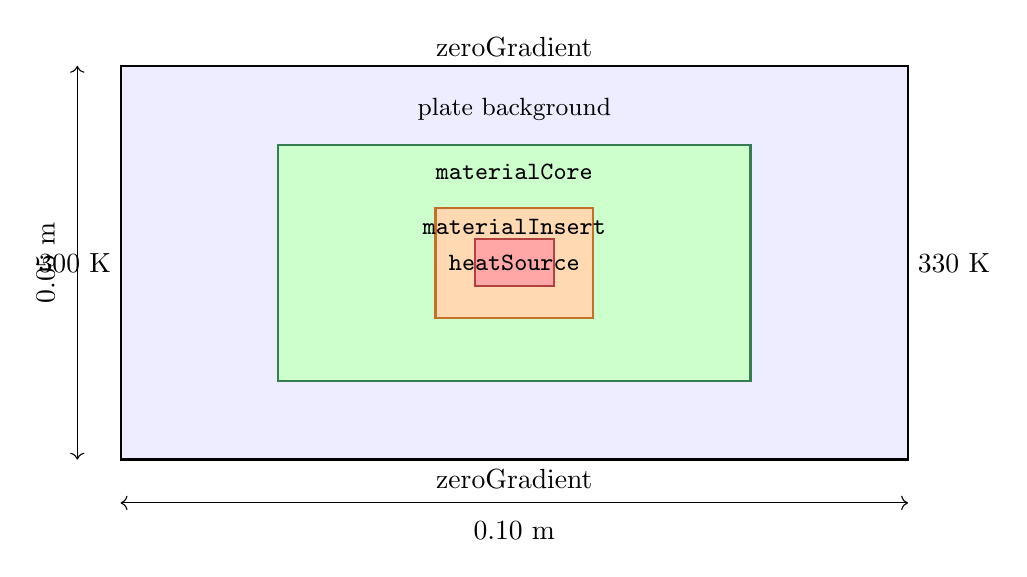
\begin{tikzpicture}[scale=1.0]
    \draw[fill=blue!7, draw=black, thick] (0,0) rectangle (10,5);
    \draw[fill=green!20, draw=foamGreen, thick] (2,1) rectangle (8,4);
    \draw[fill=orange!30, draw=foamOrange, thick] (4,1.8) rectangle (6,3.2);
    \draw[fill=red!35, draw=foamRed, thick] (4.5,2.2) rectangle (5.5,2.8);

    \node[anchor=east] at (0,2.5) {300 K};
    \node[anchor=west] at (10,2.5) {330 K};
    \node[anchor=south] at (5,5) {zeroGradient};
    \node[anchor=north] at (5,0) {zeroGradient};

    \node at (5,4.45) {\small plate background};
    \node at (5,3.65) {\small \code{materialCore}};
    \node at (5,2.95) {\small \code{materialInsert}};
    \node at (5,2.5) {\small \code{heatSource}};

    \draw[<->] (0,-0.55) -- (10,-0.55);
    \node at (5,-0.9) {$0.10~\mathrm{m}$};
    \draw[<->] (-0.55,0) -- (-0.55,5);
    \node[rotate=90] at (-0.95,2.5) {$0.05~\mathrm{m}$};
\end{tikzpicture}
\caption{Schematic of the tutorial plate. The actual OpenFOAM mesh has
100 cells in $x$, 50 cells in $y$, and one empty cell layer in $z$.}
\label{fig:tutorial-plate}
\end{figure}

\section{Physical Theory}

\subsection{Temperature and Heat Flux}

Temperature $T$ is the unknown field. Heat flux $\heatflux$ describes the rate
and direction of heat flow through a unit area. Fourier's law for anisotropic
materials is

\[
\heatflux = -\kappatensor \grad T.
\]

The minus sign is important. The temperature gradient $\grad T$ points toward
increasing temperature, but heat naturally flows from hot regions to cold
regions. Therefore the heat flux points in the opposite direction after being
scaled and rotated by the conductivity tensor.

\subsection{Energy Balance}

The solver uses the transient heat conduction equation

\[
\rho C_p \ddt{T} = \divergence \left(\kappatensor \grad T\right) + Q.
\]

In the code and input files, $\rho C_p$ is named \code{rhoCp}. It is the
volumetric heat capacity. It tells the solver how much energy is needed to
increase the temperature of one cubic meter of material by one kelvin.

\begin{table}[h]
\centering
\begin{tabularx}{\textwidth}{l l l Y}
\toprule
Symbol & OpenFOAM field & SI unit & Meaning \\
\midrule
$T$ & \code{T} & K & Temperature. This is the solved scalar field. \\
$\kappa$ & \code{kappa} & W/(m K) & Symmetric thermal conductivity tensor. \\
$\rho C_p$ & \code{rhoCp} & J/(m$^3$ K) & Volumetric heat capacity. \\
$Q$ & \code{fvOptions} & W/m$^3$ & Optional volumetric heat generation. \\
$\boldsymbol{q}$ & \code{q} & W/m$^2$ & Conductive heat flux written by the solver. \\
\bottomrule
\end{tabularx}
\caption{Main physical quantities used by the solver.}
\label{tab:physical-quantities}
\end{table}

\subsection{What Anisotropy Means}

In OpenFOAM, a symmetric tensor field is written with six components:

\[
(\kappa_{xx}\ \kappa_{xy}\ \kappa_{xz}\ \kappa_{yy}\ \kappa_{yz}\ \kappa_{zz}).
\]

For example, the tutorial background material uses

\begin{lstlisting}
internalField   uniform (1.0 0 0 0.3 0 0.3);
\end{lstlisting}

which means

\[
\kappatensor =
\begin{bmatrix}
1.0 & 0 & 0 \\
0 & 0.3 & 0 \\
0 & 0 & 0.3
\end{bmatrix}.
\]

This material conducts heat more easily in the $x$ direction than in the $y$ or
$z$ directions. The tutorial insert material instead uses

\[
\kappatensor =
\begin{bmatrix}
0.4 & 0 & 0 \\
0 & 3.0 & 0 \\
0 & 0 & 0.4
\end{bmatrix},
\]

so heat moves more easily in the $y$ direction inside the insert.

\section{Finite Volume View}

OpenFOAM uses the finite volume method. The mesh divides the domain into many
small control volumes called cells. For each cell, the solver balances the heat
stored in the cell, the heat conducted through its faces, and any internal heat
generation.

For a beginner, the most useful interpretation is:

\begin{itemize}
    \item \code{fvm::ddt(rhoCp, T)} builds the transient heat storage term.
    \item \code{fvm::laplacian(kappa, T)} builds the diffusion term caused by
    anisotropic thermal conductivity.
    \item \code{fvOptions(rhoCp, T)} adds optional source terms, such as
    volumetric heat generation in a selected cell zone.
\end{itemize}

The algebraic equation solved at every time step is assembled from

\begin{lstlisting}[language=C++]
fvScalarMatrix TEqn
(
    fvm::ddt(rhoCp, T) - fvm::laplacian(kappa, T)
 ==
    fvOptions(rhoCp, T)
);

fvOptions.constrain(TEqn);
TEqn.solve();
fvOptions.correct(T);
\end{lstlisting}

The code writes derived fields only at output times. The gradient and heat flux
are computed as

\begin{lstlisting}[language=C++]
volVectorField gradT(..., fvc::grad(T));
volVectorField q(..., (-kappa & gradT));
\end{lstlisting}

\section{Implementation Layout}

The solver intentionally uses a small OpenFOAM application layout. The key files
are listed in Table~\ref{tab:source-files}.

\begin{table}[h]
\centering
\begin{tabularx}{\textwidth}{l Y}
\toprule
File & Responsibility \\
\midrule
\code{anisotropicLaplacianFoam.C} & Main program, time loop, non-orthogonal
correction loop, equation assembly, and solve call. \\
\code{createFields.H} & Reads \code{T}, \code{kappa}, and \code{rhoCp}; creates
\code{fvOptions}. \\
\code{write.H} & Writes \code{gradT} and \code{q} at OpenFOAM write times. \\
\code{Make/files} & Defines the solver source and executable name. \\
\code{Make/options} & Defines include paths and OpenFOAM libraries. \\
\bottomrule
\end{tabularx}
\caption{Source files in the solver.}
\label{tab:source-files}
\end{table}

\subsection{Fields Read by \code{createFields.H}}

The solver requires three volume fields in the case time directory, normally
\code{0/}. Their OpenFOAM dimensions are shown in Table~\ref{tab:required-fields}.

\begin{table}[h]
\centering
\begin{tabularx}{\textwidth}{l l l Y}
\toprule
Field & OpenFOAM class & Dimensions & Meaning \\
\midrule
\code{T} & \code{volScalarField} & \code{[0 0 0 1 0 0 0]} &
Temperature in kelvin. \\
\code{kappa} & \code{volSymmTensorField} & \code{[1 1 -3 -1 0 0 0]} &
Thermal conductivity tensor in W/(m K). \\
\code{rhoCp} & \code{volScalarField} & \code{[1 -1 -2 -1 0 0 0]} &
Volumetric heat capacity in J/(m$^3$ K). \\
\bottomrule
\end{tabularx}
\caption{Required input fields.}
\label{tab:required-fields}
\end{table}

\subsection{Fields Written by \code{write.H}}

At every write time, the solver writes the fields in
Table~\ref{tab:output-fields}. These files appear in time directories such as
\code{0.5/}, \code{1/}, and \code{5/}, depending on the case settings.

\begin{table}[h]
\centering
\begin{tabularx}{\textwidth}{l l Y}
\toprule
Field & OpenFOAM class & Meaning \\
\midrule
\code{T} & \code{volScalarField} & Solved temperature field. \\
\code{gradT} & \code{volVectorField} & Temperature gradient $\grad T$. \\
\code{q} & \code{volVectorField} & Conductive heat flux
$\heatflux=-\kappatensor\grad T$. \\
\bottomrule
\end{tabularx}
\caption{Output fields expected from a successful run.}
\label{tab:output-fields}
\end{table}

\section{Build and Run Workflow}

\subsection{Build the Solver}

Source the OpenFOAM v2512 environment first. The exact command depends on the
local installation. After the environment is active, build from the repository
root:

\begin{lstlisting}[language=bash]
cd /path/to/anisotropicLaplacianFoam
wmake
\end{lstlisting}

The executable is installed as
\code{\$(FOAM\_USER\_APPBIN)/anisotropicLaplacianFoam}, as specified by
\code{Make/files}.

\subsection{Run the Tutorial}

The tutorial can be run with the provided script:

\begin{lstlisting}[language=bash]
cd tutorials/compositePlate2D
./Allrun
\end{lstlisting}

The script performs the same workflow shown in Figure~\ref{fig:workflow}.

\begin{figure}[h]
\centering
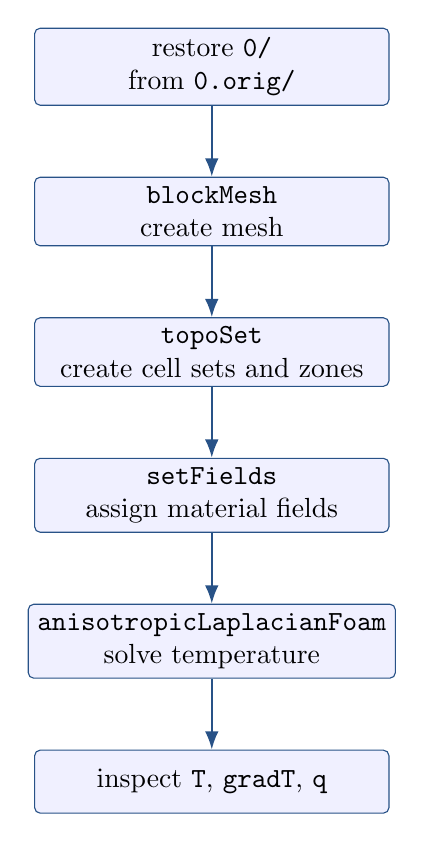
\begin{tikzpicture}[
    node distance=9mm,
    flowStep/.style={
        rectangle,
        rounded corners=2pt,
        draw=foamBlue,
        fill=blue!6,
        minimum width=45mm,
        minimum height=8mm,
        align=center
    },
    arrow/.style={-Latex, thick, draw=foamBlue}
]
    \node[flowStep] (restore) {restore \code{0/}\\from \code{0.orig/}};
    \node[flowStep, below=of restore] (mesh) {\code{blockMesh}\\create mesh};
    \node[flowStep, below=of mesh] (topo) {\code{topoSet}\\create cell sets and zones};
    \node[flowStep, below=of topo] (fields) {\code{setFields}\\assign material fields};
    \node[flowStep, below=of fields] (solve) {\code{anisotropicLaplacianFoam}\\solve temperature};
    \node[flowStep, below=of solve] (view) {inspect \code{T}, \code{gradT}, \code{q}};

    \draw[arrow] (restore) -- (mesh);
    \draw[arrow] (mesh) -- (topo);
    \draw[arrow] (topo) -- (fields);
    \draw[arrow] (fields) -- (solve);
    \draw[arrow] (solve) -- (view);
\end{tikzpicture}
\caption{Tutorial execution workflow.}
\label{fig:workflow}
\end{figure}

The manual equivalent is:

\begin{lstlisting}[language=bash]
cd tutorials/compositePlate2D
rm -rf 0
cp -r 0.orig 0
blockMesh
topoSet
setFields
anisotropicLaplacianFoam
\end{lstlisting}

\section{Tutorial Case Details}

\subsection{Mesh}

The file \code{tutorials/compositePlate2D/system/blockMeshDict} creates a
rectangular plate:

\begin{itemize}
    \item length: $0.10~\mathrm{m}$,
    \item height: $0.05~\mathrm{m}$,
    \item thickness: $0.001~\mathrm{m}$,
    \item cells: $100 \times 50 \times 1$.
\end{itemize}

The front and back patches use the OpenFOAM \code{empty} boundary type. This is
how a geometrically thin 3D mesh is treated as a 2D calculation.

\subsection{Boundary Conditions}

The initial temperature field is stored in \code{0.orig/T}. The boundary
conditions are:

\begin{table}[h]
\centering
\begin{tabularx}{\textwidth}{l l Y}
\toprule
Patch & Boundary condition & Meaning \\
\midrule
\code{left} & \code{fixedValue}, 300 K & Cold side of the plate. \\
\code{right} & \code{fixedValue}, 330 K & Hot side of the plate. \\
\code{bottom} & \code{zeroGradient} & Insulated boundary. \\
\code{top} & \code{zeroGradient} & Insulated boundary. \\
\code{frontAndBack} & \code{empty} & 2D front and back patches. \\
\bottomrule
\end{tabularx}
\caption{Tutorial temperature boundary conditions.}
\label{tab:boundary-conditions}
\end{table}

\subsection{Material Regions}

\code{topoSet} creates three cell zones:

\begin{itemize}
    \item \code{materialCore}: a rectangular core region,
    \item \code{materialInsert}: a smaller insert inside the core,
    \item \code{heatSource}: a small source region inside the insert.
\end{itemize}

\code{setFields} assigns material properties. If a cell is not inside one of
the listed regions, it keeps the default background values.

\begin{table}[h]
\centering
\begin{tabularx}{\textwidth}{l l l Y}
\toprule
Region & Approximate box in $(x,y)$ & \code{rhoCp} & \code{kappa} components \\
\midrule
background & rest of plate & $2.0\times10^6$ &
$(1.0,0,0,0.3,0,0.3)$ \\
\code{materialCore} & $(0.02,0.01)$ to $(0.08,0.04)$ & $2.4\times10^6$ &
$(8.0,0,0,0.8,0,0.8)$ \\
\code{materialInsert} & $(0.04,0.018)$ to $(0.06,0.032)$ & $1.6\times10^6$ &
$(0.4,0,0,3.0,0,0.4)$ \\
\bottomrule
\end{tabularx}
\caption{Material properties assigned by \code{setFieldsDict}. Conductivity
components are ordered as $(xx,xy,xz,yy,yz,zz)$.}
\label{tab:material-regions}
\end{table}

\subsection{Internal Heat Generation}

The file \code{system/fvOptions} defines a source named \code{heatGeneration}.
Its option type, selected cell zone, and source values are:

\begin{lstlisting}
heatGeneration
{
    type            scalarSemiImplicitSource;
    active          yes;

    selectionMode   cellZone;
    cellZone        heatSource;
    volumeMode      specific;

    injectionRateSuSp
    {
        T           (1.0e6 0);
    }
}
\end{lstlisting}

The first value is the explicit source coefficient. The second value is the
implicit coefficient. In this tutorial the implicit coefficient is zero, so the
source behaves as a prescribed heat generation term in the selected zone.

\subsection{Time Controls}

\code{system/controlDict} runs from $t=0$ to $t=5$ with a time step of
$\Delta t=0.01$. It writes results every 0.5 seconds of simulated time:

\begin{lstlisting}
endTime         5;
deltaT          0.01;
writeControl    runTime;
writeInterval   0.5;
\end{lstlisting}

\section{Inspecting Results}

After a successful run, open the case with ParaView or another OpenFOAM-capable
post-processor. Useful first checks are:

\begin{itemize}
    \item Plot \code{T}. It should remain near the imposed 300 K and 330 K
    boundary values while being modified by internal heat generation.
    \item Plot \code{gradT}. It shows where temperature changes most rapidly.
    \item Plot \code{q} as vectors. The vectors show the conductive heat flux
    direction and magnitude.
    \item Compare \code{q} direction in different materials. An anisotropic
    insert can redirect heat flow even when the temperature contours look
    smooth.
\end{itemize}

\section{Common Problems}

\begin{table}[h]
\centering
\begin{tabularx}{\textwidth}{l Y Y}
\toprule
Symptom & Likely cause & Check \\
\midrule
\code{Unknown application} & The solver has not been built or the OpenFOAM
environment is not sourced. & Run \code{wmake} from the repository root and
check that \code{FOAM\_USER\_APPBIN} is in \code{PATH}. \\
Missing \code{kappa} or \code{rhoCp} & The case \code{0/} directory was not
created from \code{0.orig/}. & Run \code{rm -rf 0 \&\& cp -r 0.orig 0}. \\
Patch type error for 2D case & One field does not use \code{empty} on
\code{frontAndBack}. & Check \code{T}, \code{kappa}, and \code{rhoCp}. \\
No heat source effect & \code{topoSet} or \code{fvOptions} did not create or
select \code{heatSource}. & Run \code{topoSet}; inspect
\texttt{constant/polyMesh/\allowbreak cellZones}. \\
Unexpected heat flux direction & Sign convention misunderstood. &
Remember that \code{q = -kappa \& gradT}; heat flows from hot to cold. \\
\bottomrule
\end{tabularx}
\caption{Beginner troubleshooting checklist.}
\label{tab:troubleshooting}
\end{table}

\section{Minimal Checklist for a New Case}

To create a new case for this solver:

\begin{enumerate}
    \item Create a mesh with valid boundary patches.
    \item Provide \code{0/T}, \code{0/kappa}, and \code{0/rhoCp}.
    \item Use \code{volSymmTensorField} for \code{kappa}.
    \item Use dimensions \code{[1 1 -3 -1 0 0 0]} for \code{kappa}.
    \item Use dimensions \code{[1 -1 -2 -1 0 0 0]} for \code{rhoCp}.
    \item Add \code{fvOptions} only if an internal heat source is needed.
    \item Set \code{application anisotropicLaplacianFoam;} in
    \code{system/controlDict}.
    \item Run the solver and inspect \code{T}, \code{gradT}, and \code{q}.
\end{enumerate}

\section{Summary}

\code{anisotropicLaplacianFoam} solves transient heat conduction in stationary
solids using physical material properties. The required model is compact:
\code{T} is the unknown, \code{kappa} controls directional heat conduction, and
\code{rhoCp} controls transient heat storage. The tutorial demonstrates the full
workflow: create the mesh, create material zones, assign fields, solve, and
inspect temperature gradient and heat flux.

\end{document}
